\subsection{Solar radiation perturbation}
The below equation shows the force of solar radiation.
$$
P_{SRP} = \nu \dfrac{S}{c}C_R \dfrac{A_s}{m}
$$
where $\nu$ calculates if the satellite is in the earth's shadow or not.
Then used the below equations for rate changes.

\begin{figure}[H]
    \centering
    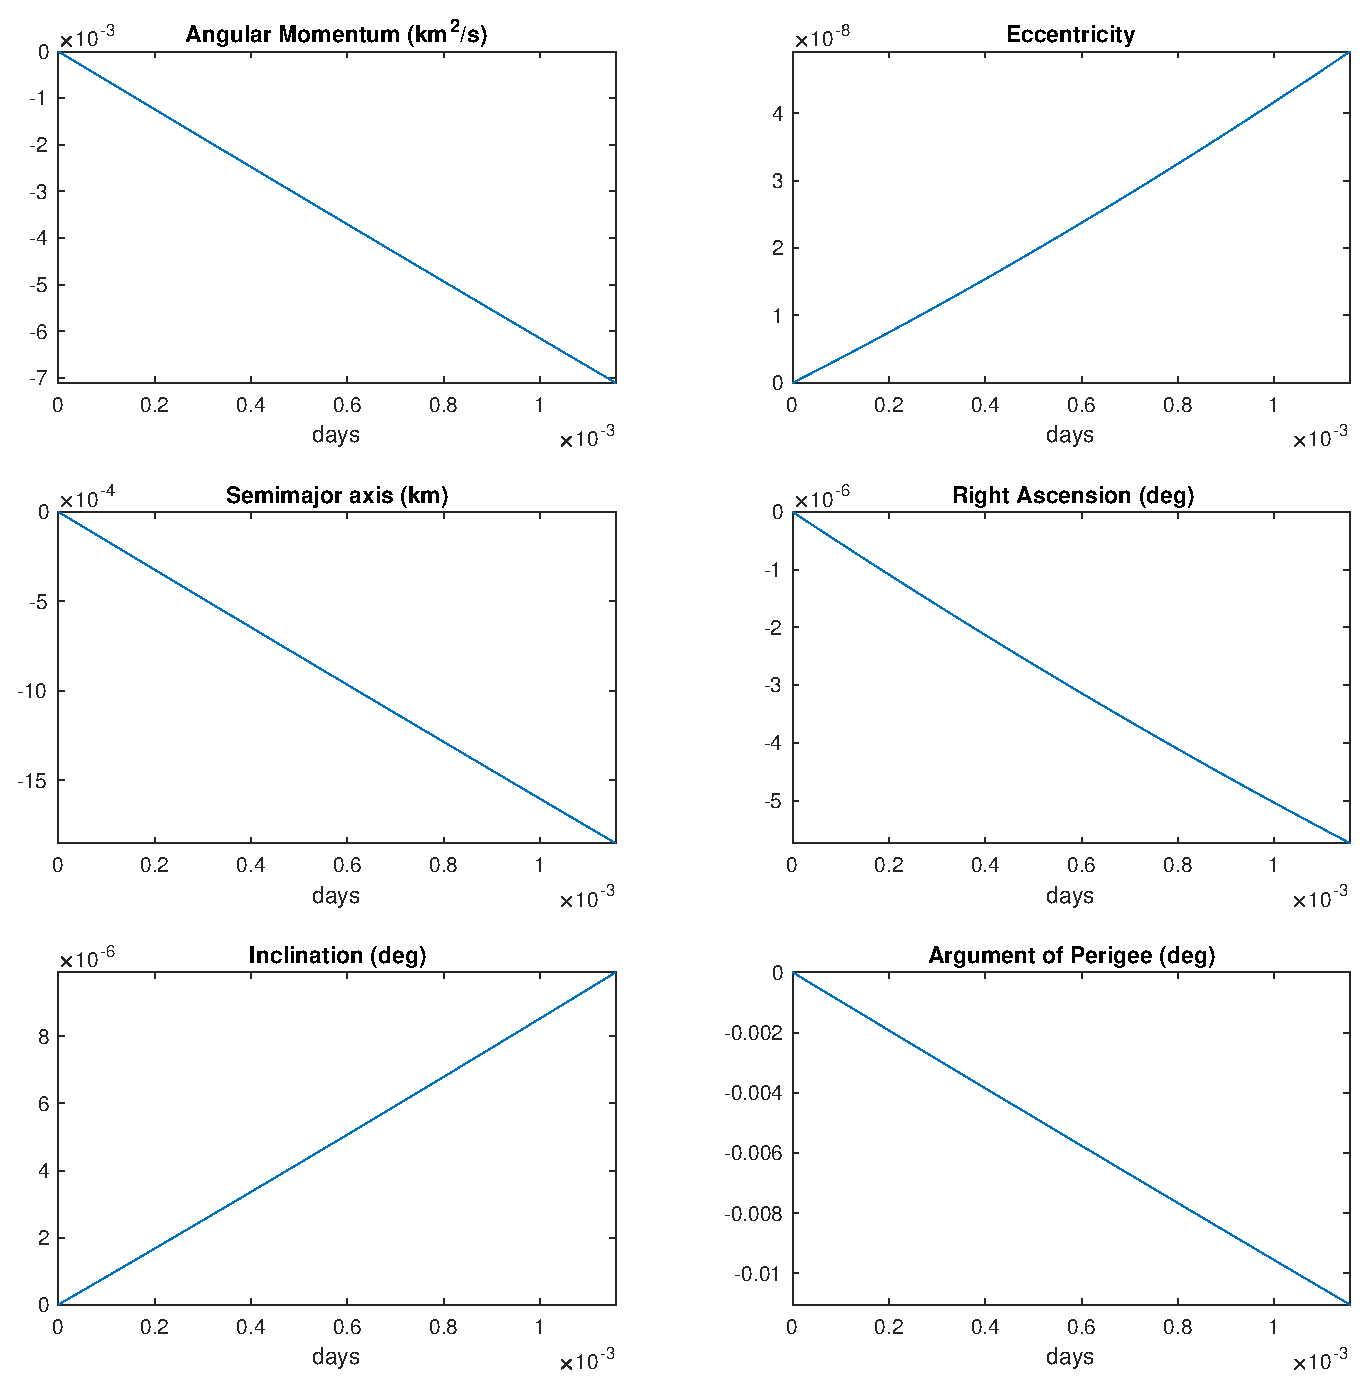
\includegraphics[width=0.85\textwidth]{../Figure/Q2/e_100}
    \caption{Variation of Parameter due to solar radiation perturbation for 100 seconds}
\end{figure}

\begin{figure}[H]
    \centering
    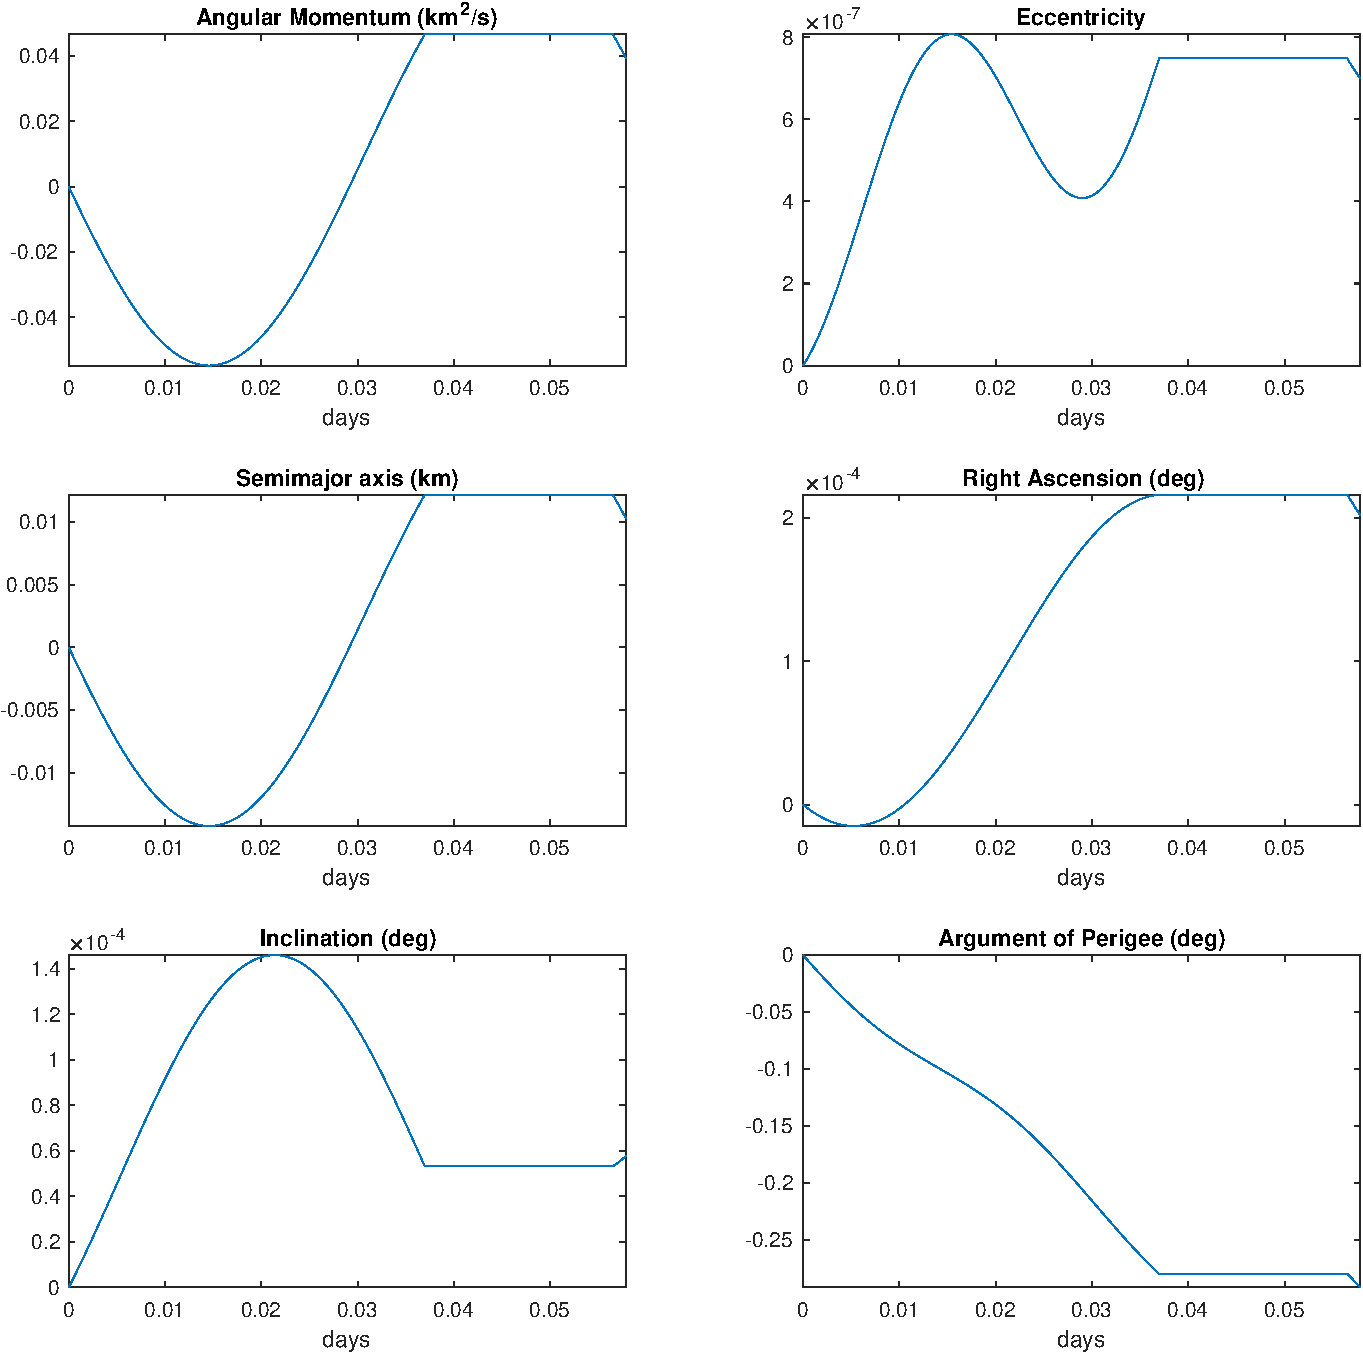
\includegraphics[width=0.85\textwidth]{../Figure/Q2/e_5000}
    \caption{Variation of Parameter due to solar radiation perturbation for 5000 seconds}
\end{figure}

\begin{figure}[H]
    \centering
    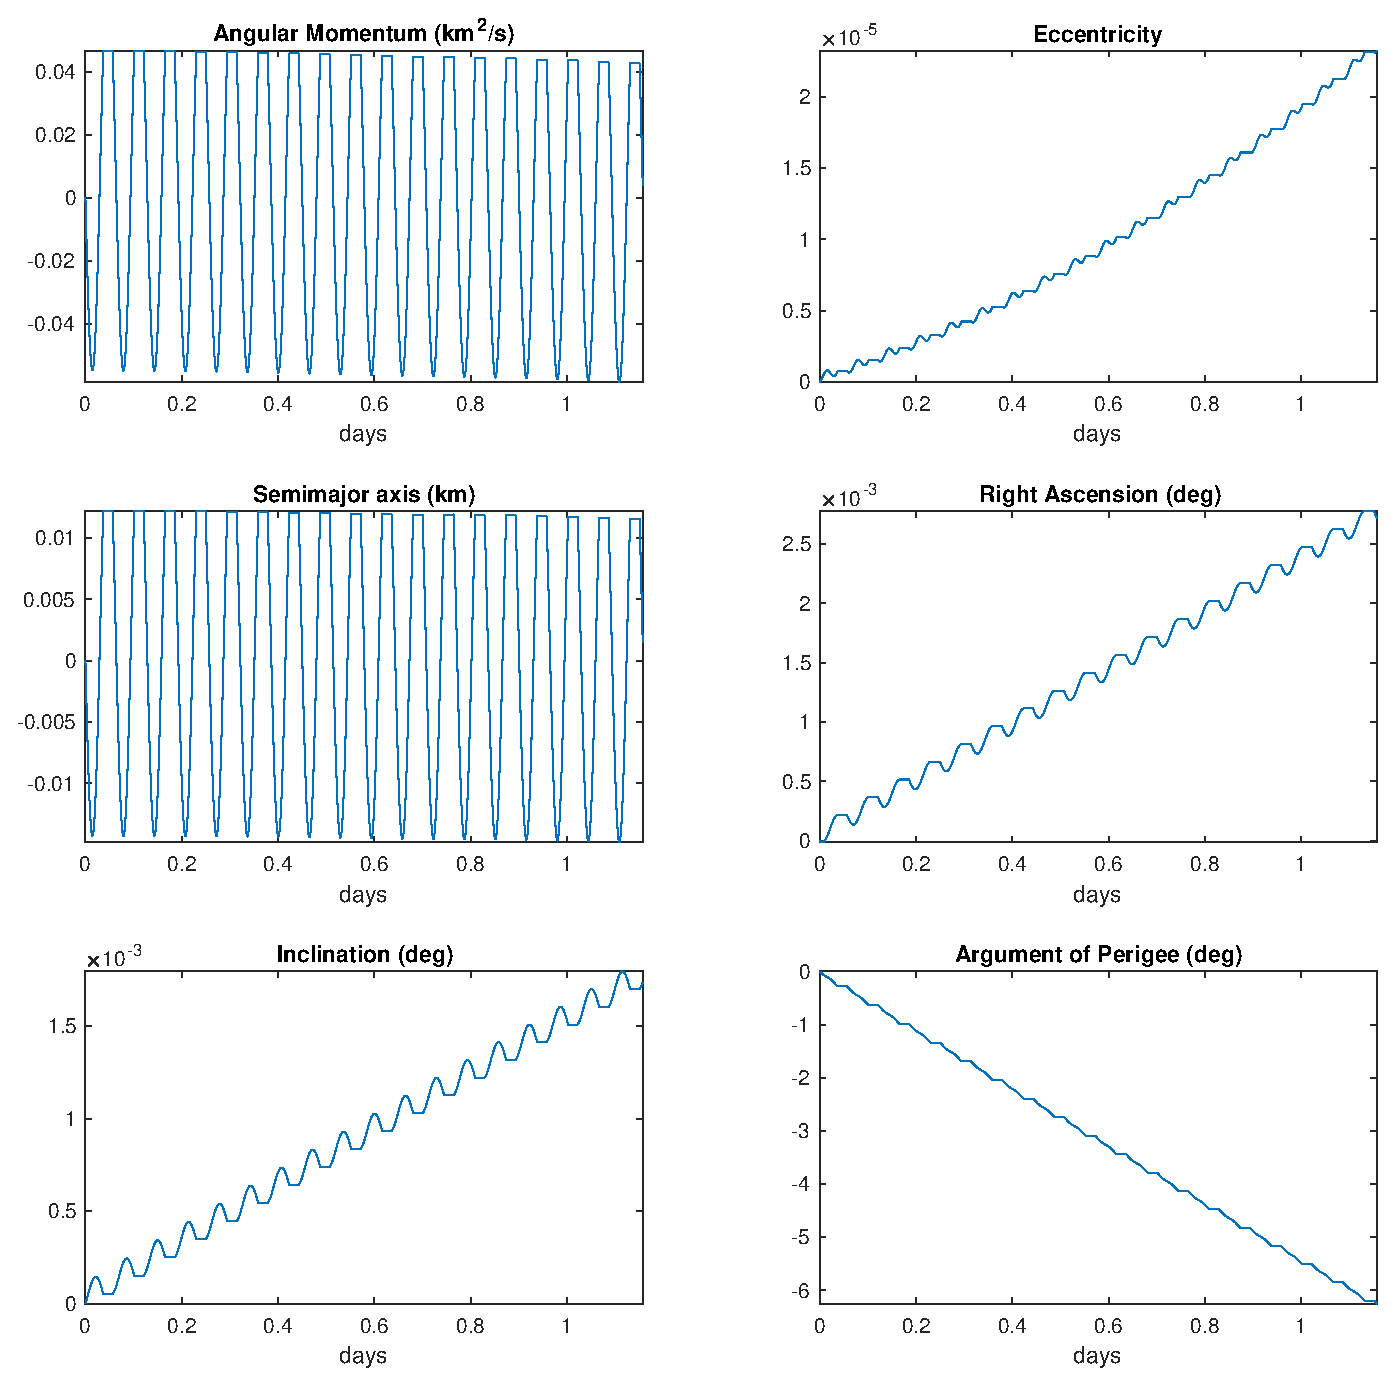
\includegraphics[width=0.85\textwidth]{../Figure/Q2/e_100000}
    \caption{Variation of Parameter due to solar radiation perturbation for 100000 seconds}
\end{figure}